\documentclass{standalone}

\usepackage[OT1]{fontenc}
\renewcommand*\familydefault{\sfdefault}
\usepackage{helvet,sfmath}
\usepackage{siunitx}

\usepackage{tikz}
\usetikzlibrary{arrows,calc,patterns}
\usepackage{tikz,tkz-euclide}

\definecolor{BlueDefault}{rgb}{0.2,0.2,0.7}

\begin{document}

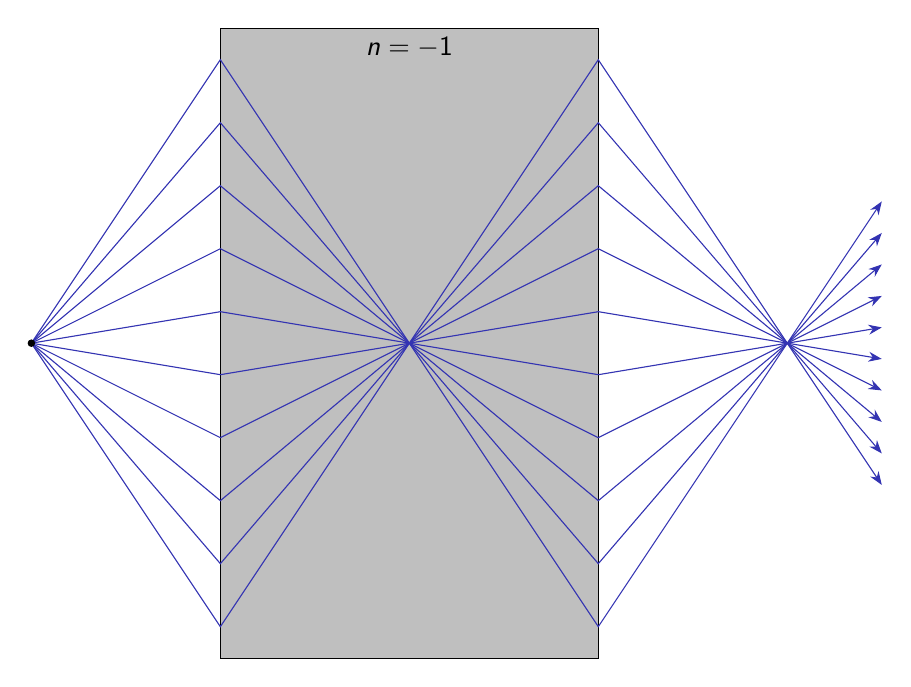
\begin{tikzpicture}[scale=0.8]
    %%Lens
    \draw[fill=lightgray] (-3,-5) to (3,-5) to (3,5) to (-3,5) to (-3,-5);
    \foreach \x in {-4.5,-3.5,...,4.5}
    {
    \draw[BlueDefault, -Stealth] (-6,0) to (-3,\x) to (3,-\x) to (7.5,0.5*\x);
    }
    \draw[fill=black] (-6,0) circle (0.05);
    \draw (0,4.7) node{\(n=-1\)};
\end{tikzpicture}

\end{document}